\documentclass[10pt,a4paper]{article}
\usepackage[margin=20mm]{geometry}
\usepackage[T1]{fontenc}
\usepackage{lmodern,microtype,graphicx,booktabs,tabularx,xcolor}
\usepackage[colorlinks=true,urlcolor=teal,linkcolor=teal]{hyperref}
\setlength{\parindent}{0pt}
\setlength{\parskip}{6pt}
\definecolor{ink}{HTML}{202D4D}
\newcommand{\code}[1]{\texttt{\small #1}}
\hypersetup{pdftitle={Alpha Compiler and Virtual Machine: Technical Brief},pdfauthor={Dimitris Asimakopoulos, Alexandros Fourtounis, Georgia Marina Tsanta}}
\begin{document}
{\color{ink}\LARGE\bfseries Alpha Compiler \& Virtual Machine}\par
{\large Technical brief}\hfill HY340, University of Crete, 2023--2024\par
{\small Dimitris Asimakopoulos \enspace\textperiodcentered\enspace Alexandros Fourtounis \enspace\textperiodcentered\enspace Georgia Marina Tsanta}

\section*{1\quad From source code to bytecode}
Alpha is a course compiler implemented in C with Flex and Bison. The final integrated implementation combines lexical and syntax analysis, symbol management, three-address intermediate code, target-code generation, and a companion Alpha Virtual Machine (AVM). The work is jointly authored, and the supplied MIT license is preserved.

\begin{center}
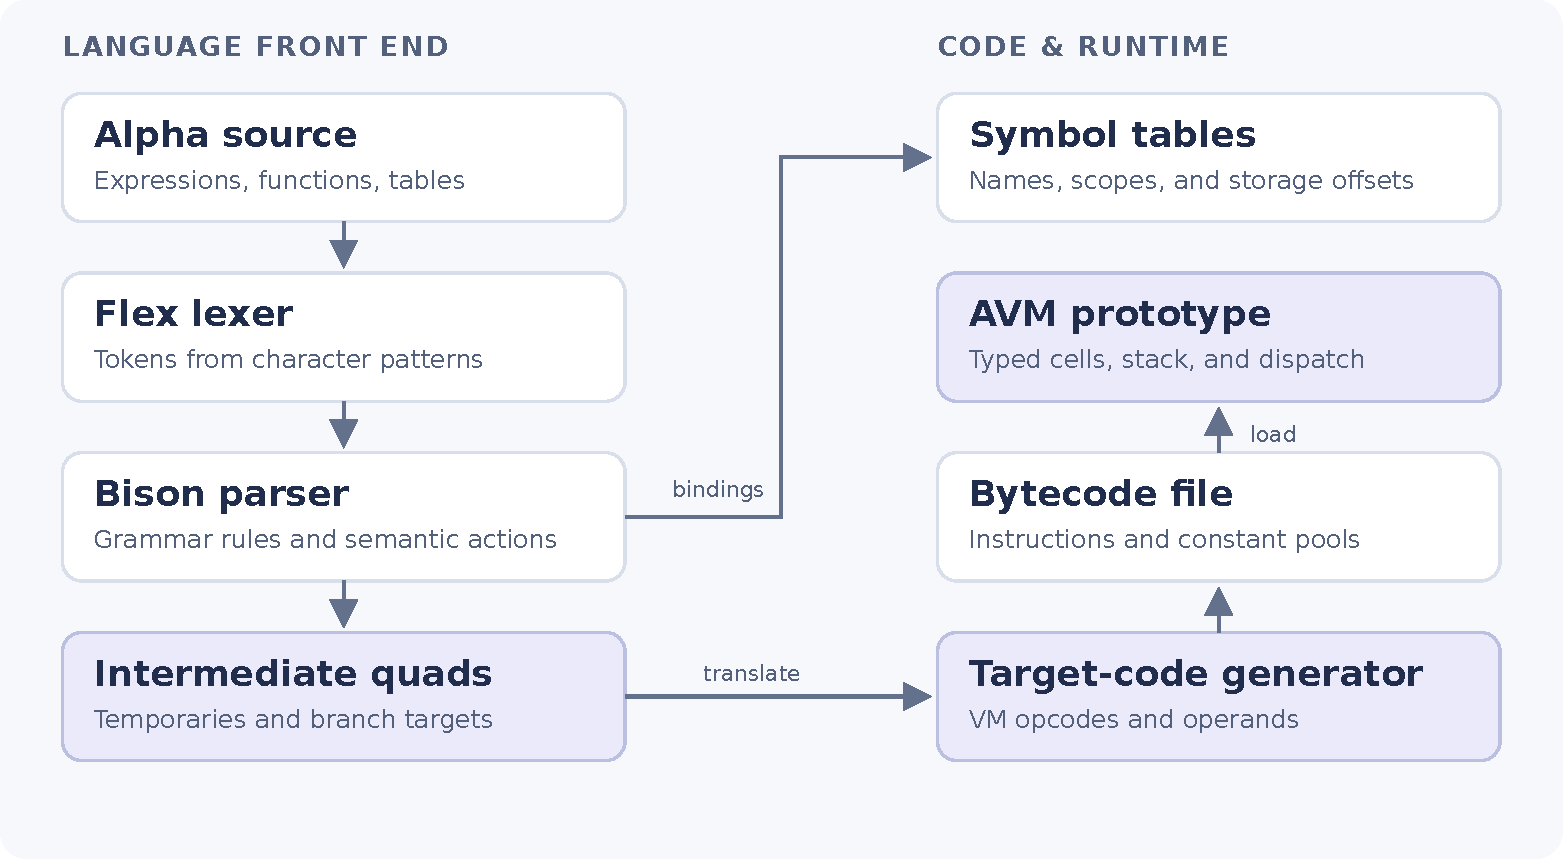
\includegraphics[width=0.96\linewidth]{assets/architecture.pdf}
\end{center}
\vspace{-7pt}
{\small\textbf{Figure 1.} The compiler exports intermediate and target representations. The AVM is an experimental runtime and is not a verified execution backend.}

\textbf{Front end.} Flex patterns recognize keywords, names, literals, punctuation, and operators. Bison grammar actions process expressions, blocks, conditional statements, loops, functions, calls, and table expressions. Symbol entries distinguish global, local, and formal variables from user and library functions. Hash lookup and per-scope links support name tracking, while storage-space offsets prepare variables for target operands.

\textbf{Intermediate representation.} Semantic actions emit quads containing an opcode, result, arguments, branch label, and source line. Temporary symbols hold intermediate expression values. Branch lists and patching helpers represent control-flow targets that become known later. This representation separates language-level operations from VM instruction encoding without requiring a separate abstract syntax tree.

\textbf{Back end.} Generator functions map quad operations to VM opcodes and operands. Separate pools hold numeric and string constants, library names, and user-function metadata. Readable quad and instruction listings expose the translation before serialization, making it possible to inspect a program without executing the VM.

\newpage
\section*{2\quad Runtime design and implementation boundaries}
The AVM uses a 4,096-cell stack with tagged values for numbers, strings, booleans, tables, functions, nil, and undefined values. Operand translation distinguishes globals, locals, formals, constants, and the return-value cell. An opcode dispatch table connects instructions to execution handlers. Call frames store the argument count, return program counter, and saved stack positions. Tables use typed hash buckets and reference counters.

These structures demonstrate the connection between compiler storage decisions and runtime behavior. They remain a course implementation with material limitations:

\begin{tabularx}{\linewidth}{@{}p{0.23\linewidth}X@{}}
\toprule
\textbf{Area} & \textbf{Current implementation} \\
\midrule
Control flow & Backpatching is implemented, but some paths remain incomplete. In the VM, unconditional jumps dispatch to a no-op and logical handlers contain assertions. \\
Constant operands & The numeric-pool insertion helper returns the numeric value rather than its pool index. The demo therefore emits numeric operands that cannot be interpreted as valid pool references. \\
Binary representation & Serialization uses native enums, \code{size\_t}, and operand-sized memory blocks. It is tied to the host layout and is not a portable bytecode specification. \\
Execution & The arithmetic demo aborts in a VM stack assertion. Successful file generation does not establish correct end-to-end program execution. \\
Diagnostics & Parse errors are printed, but the compiler entry point does not reliably propagate them through its exit status. \\
\bottomrule
\end{tabularx}

\section*{3\quad Verification and reproduction}
The integrated compiler and VM build with GCC 13.3, Flex 2.6.4, Bison 3.8.2, and GNU Make 4.3 on Linux. The compiler retains warnings and the grammar reports two shift/reduce conflicts. Instruction slot zero is reserved and initialized before generation. Build products are kept outside the source directories.

\textbf{Compiler example.} The included program assigns 6 and 7, multiplies the variables, and calls \code{print}. Compilation produces 10 quads and 10 serialized instructions, plus numeric constants and a library-function entry. The demonstration displays these artifacts and does not execute the experimental runtime.

\textbf{Focused checks.} Automated checks inspect the variable-multiplication quad and print-call instruction, verify literal addition operands, read the string and number pools independently, and compare the serialized payload size against the instruction listing using the host operand layout. A malformed input checks syntax-error reporting. Temporary paths contain spaces to exercise file handling. These checks cover selected compiler outputs and binary framing, not complete language semantics or VM correctness.

From the repository root, \code{make} builds both executables, \code{make demo} runs the compilation example, and \code{make check} runs the focused checks. The setup guide documents artifact locations and the VM's working-directory expectation. Historical factorial, Fibonacci, conditional, and loop inputs are retained for inspection, without claiming they execute correctly.

The older lexical and syntax assignment PDFs supplied with the project describe the course context. The current grammar and C implementation are the basis for this brief. The main engineering contribution is the integration of parsing, scoped symbols, intermediate representations, bytecode data structures, and a runtime model.
\end{document}
